\documentclass[10pt,twoside]{tenth}

\usepackage[norndcorners,customcolors]{hf-tikz}
\hfsetbordercolor{Yellow3!50}
\hfsetfillcolor{Yellow2!30}

% !TEX root = report.tex
%%--------------------------------------------
%%  Define Alloy syntax for highlighting
%%--------------------------------------------
\lstdefinelanguage{alloy}{%
    morekeywords=[1]{%
        abstract,all,and,as,assert,but,check,disj,else,enum,exactly,expect,%
        extends,fact,for,fun,iden,iff,implies,in,Int,int,let,lone,module,no,%
        none,not,one,open,or,pred,private,run,seq,set,sig,some,sum,this,univ},%
    morekeywords=[2]{%
        plus,minus,mul,div,rem,elems,first,last,rest,butlast,isEmpty,hasDups,%
        inds,lastIdx,afterLastIdx,idxOf,lastIdxOf,indsOf,add,setAt,insert,
        delete,append,subseq},%
    literate=*%
        %% Single character
        {:}{{{\bfseries\color{Symbol}{:}}}}1
        {@}{{{\color{Symbol}{@}}}}1
        {!}{{{\color{Symbol}{!}}}}1
        {\#}{{{\color{Symbol}{\#}}}}1
        {\~}{{{\color{Symbol}{\~}}}}1
        {*}{{{\color{Symbol}{*}}}}1
        {\^}{{{\color{Symbol}{\^}}}}1
        {\&}{{{\color{Symbol}{\&}}}}1  % combined
        {+}{{{\color{Symbol}{+}}}}1  % combined
        {-}{{{\color{Symbol}{-}}}}1
        {.}{{{\bfseries\color{Symbol}{.}}}}1
        {=}{{{\color{Symbol}{=}}}}1
        {<}{{{\color{Symbol}{<}}}}1
        {>}{{{\color{Symbol}{>}}}}1
        {|}{{{\bfseries\color{Symbol}{|}}}}1
        %% Double characters
        {||}{{{\color{Symbol}{||}}}}1  % combined special
        {\&\&}{{{\color{Symbol}{\&\&}}}}1  % combined special
        {=>}{{{\color{Symbol}{=>}}}}2  % combined
        {++}{{{\color{Symbol}{++}}}}2
        {<:}{{{\color{Symbol}{<:}}}}2
        {:>}{{{\color{Symbol}{:>}}}}2
        {=<}{{{\color{Symbol}{=<}}}}1  % combined
        {>=}{{{\color{Symbol}{>=}}}}1  % combined
        {->}{{{\color{Symbol}{->}}}}2  % special
        {!=}{{{\color{Symbol}{!=}}}}1  % special
        %% Triple characters
        {<=>}{{{\color{Symbol}{<=>}}}}2  % combined
        ,
    % literate=*%
    %     %% Single character
    %     {:}{{{\bfseries\color{Symbol}{:}}}}1
    %     {@}{{{\color{Symbol}{@}}}}1
    %     {!}{{{\color{Symbol}{!}}}}1
    %     {\#}{{{\color{Symbol}{\#}}}}1
    %     {\~}{{{\color{Symbol}{\~}}}}1
    %     {*}{{{\color{Symbol}{*}}}}1
    %     {\^}{{{\color{Symbol}{\^}}}}1
    %     {\&}{{{\color{Symbol}{$\cap$}}}}1  % combined
    %     {+}{{{\color{Symbol}{$\cup$}}}}1  % combined
    %     {-}{{{\color{Symbol}{-}}}}1
    %     {.}{{{\bfseries\color{Symbol}{.}}}}1
    %     {=}{{{\color{Symbol}{=}}}}1
    %     {<}{{{\color{Symbol}{<}}}}1
    %     {>}{{{\color{Symbol}{>}}}}1
    %     {|}{{{\bfseries\color{Symbol}{|}}}}1
    %     %% Double characters
    %     {||}{{{\color{Symbol}{$\lor$}}}}1  % combined special
    %     {&&}{{{\color{Symbol}{$\land$}}}}1  % combined special
    %     {=>}{{{\color{Symbol}{$\Rightarrow$}}}}2  % combined
    %     {++}{{{\color{Symbol}{++}}}}2
    %     {<:}{{{\color{Symbol}{<:}}}}2
    %     {:>}{{{\color{Symbol}{:>}}}}2
    %     {=<}{{{\color{Symbol}{$\le$}}}}1  % combined
    %     {>=}{{{\color{Symbol}{$\ge$}}}}1  % combined
    %     {->}{{{\color{Symbol}{$\rightarrow$}}}}2  % special
    %     {!=}{{{\color{Symbol}{$\neq$}}}}1  % special
    %     %% Triple characters
    %     {<=>}{{{\color{Symbol}{$\Leftrightarrow$}}}}2  % combined
    %     ,
    alsodigit={'"},%
    identifierstyle=\color{black!80},%
    sensitive=true,%
    morecomment=[l]{//},%
    morecomment=[l]{--},%
    morecomment=[s]{/*}{*/},%
    escapeinside={<|}{|>}}

\newrobustcmd\alloy[1]{\lstinline[language=alloy]{#1}}
\newrobustcmd\alloyfn[1]{\lstinline[language=alloy,basicstyle={\ttfamily\footnotesize}]{#1}}
  % alloy syntax highlighter and set as default listing

%%--------------------------------------------
%%  Define commands
%%--------------------------------------------
\newrobustcmd{\texthyphens}{\mathcode`\-=`\-\relax}
\newrobustcmd{\id}[1]{\ensuremath{\mathit{\color{red} #1}}}  % to be removed
\newrobustcmd{\rel}[1]{\ensuremath{\text{\textnormal{\textsf{\textbf{#1}}}}}}  % relation and field names
\newrobustcmd{\field}[1]{\ensuremath{\mathsf{\texthyphens#1}}}  % relation and field names
\newrobustcmd{\var}[1]{\ensuremath{\mathit{#1}}}  % variables
\newrobustcmd{\val}[1]{\ensuremath{\text{\textnormal{\ttfamily{#1}}}}} % values
\newrobustcmd{\str}[1]{\ensuremath{\text{\textnormal{`\ttfamily{#1}}'}}} % string values

% Highlight inside lstlisting
\newrobustcmd{\hll}[1]{\makebox[0pt]{\tikzmarkin{hl:#1}(0.1,0.3)(0.0,-0.1)}}
\newrobustcmd{\hlr}[1]{{\tikzmarkend{hl:#1}}}

% Paragraph in caption
\newrobustcmd{\captionpar}{\smallskip\hspace*{2pc}}

% Variable inside code
\colorlet{CodeVariable}{rgb:Orange2,5;black,2}

%%--------------------------------------------
%%  Define document attributes
%%--------------------------------------------
\newrobustcmd\mytitle{%
    Safety Checking for Domain Relational Calculus Queries %
    Using Alloy Analyzer %
}
\newrobustcmd\myauthor{Abhabongse Janthong}

\renewrobustcmd\leftheader{%
    \adforn{34}\: safety checking for drc {q}ueries using alloy analyzer}
\renewrobustcmd\rightheader{%
    abhabongse\: janthong\: \adforn{62}}

\title{\mytitle}
\author{\myauthor}
\date{}

\begin{document}
\maketitle

\begin{abstract}
    \smallskip\setstretch{1}
    A domain relational calculus (\textsc{drc}) query is a database query which uses the mathematical set notation to enumerate the result based on the data in the database. A \textsc{drc} query is safe if and only if it is domain-independent, i.e., the result of the query is determined solely by the data in the database, not the domain of data values. In this project, we provide a framework for verifying whether a given \textsc{drc} query is safe by translating the problem into a verification task in Alloy language. We also experiment with our translation framework using various examples of safe and unsafe queries.
\end{abstract}

\begin{small}
    \tableofcontents
\end{small}
\clearpage

% !TEX root = report.tex
\section{Introduction}


\subsection{Basic definition of database system}

In database systems, a \textbf{database} is a collection of tables, and each \textbf{table} stores one coherent dataset. Each row of a table represents a single data point and each column represents an attribute of the data. Theoretically speaking, a table is merely a mathematical \textbf{relation} over one or more sets of scalar values (numbers, strings, etc.) and each row of the table is a \textbf{tuple} (or an element) in such relation.

For the sake of keeping our explanation simple, the relationship of data across different tables can be expressed by declaring \textbf{keys} (usually referred as IDs) as explicit columns in the table. Each row of a table may have a \textbf{primary key} declared as an anchor point to which other tables can refer to with \textbf{foreign keys}. In practice, since integers can be used as keys, it is sufficient to portray keys no different than other scalar values. Therefore, we omit the keys from our discussion for the rest of this project.

\smallskip
\marginhead{First example of database}
For example, let us say that we would like to construct a database to store information of four students: Alice, Bob, Carol, and David. The database must contain their personal data (e.g. year of birth) as well as a network graph representing their friendship relation. One possibility is that we create two tables, described below.

\newrobustcmd\nameA{\field{Name\hrsp{}A}}
\newrobustcmd\nameB{\field{Name\hrsp{}B}}
\newrobustcmd\personaldata{\rel{PersonalData}(\field{Name},\field{BirthYear})}
\newrobustcmd\friendship{\rel{Friendship}(\nameA,\nameB)}

\begin{itemize}[topsep=0.5pc,itemsep=0.25pc]
    \item  $\personaldata$: a two-column table containing each student's name and year of birth;
    \item  $\friendship$: a (possibly non-symmetric) two-column table where each row contains names and only names of two students who are friends of each other.
\end{itemize}
An example of an instance of such database are shown in \autoref{tab:age} and \autoref{tab:friend}, and the visualization is shown in \autoref{fig:alicebob}.

\smallskip
\begin{table}[!h]
    \small\centering
    \begin{minipage}{0.45\linewidth}
        \centering
        \begin{tabular}{ll}
            \toprule
            \field{Name} & \field{BirthYear} \\
            \midrule
            \str{Alice} & \val{1994} \\
            \str{Bob} & \val{1995} \\
            \str{Carol} & \val{1994} \\
            \str{David} & \val{1993} \\
            \bottomrule
        \end{tabular}
        \caption{Table \rel{PersonalData} with four students: Alice, Bob, Carol, and David, and their corresponding year of birth.}
        \label{tab:age}
    \end{minipage}
    \begin{minipage}{0.45\linewidth}
        \centering
        \begin{tabular}{ll}
            \toprule
            \nameA & \nameB \\
            \midrule
            \str{Alice} & \str{Bob} \\
            \str{Bob} & \str{Carol} \\
            \str{Alice} & \str{Carol} \\
            \str{Carol} & \str{David} \\
            \bottomrule
        \end{tabular}
        \caption{Table \rel{Friendship} showing that Alice, Bob, and Carol know each other, but David knows only Carol.}
        \label{tab:friend}
    \end{minipage}
\end{table}
\begin{figure}[!h]
    \small\centering
    \begin{minipage}[b]{0.35\linewidth}
        \caption{The visualization of data in the table \rel{PersonalData} and \rel{Friendship}.}
        \label{fig:alicebob}
    \end{minipage}
    \begin{minipage}[b]{0.55\linewidth}
        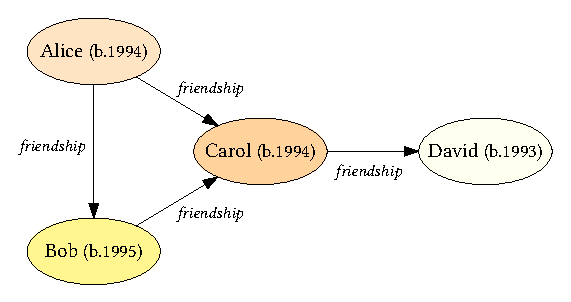
\includegraphics[width=0.8\linewidth]{figures/alicebob.eps}
    \end{minipage}
\end{figure}

\newpage
\subsection{Database query model}

One of the most basic database function is the \textbf{query} function, i.e., the process of fetching the stored data from the database. SQL model is an example of one of the most practical query model adopted in industry. Nonetheless, it is also useful to discuss theoretical query models (such as \textbf{relational calculus} and \textbf{relational algebra}) in order to gain a better understanding of database query models.

\marginhead{Definition of Domain Relational Calculus}In this report, we mainly discuss one particular variant of relational calculus query model, namely the \textbf{domain relational calculus} (\textsc{drc}). In this model,
\begin{itemize}[topsep=0.5pc,itemsep=0.25pc]
    \item  We use set comprehension notation (i.e., set defined by a predicate) to construct a query result. Such predicate must be in first-order logic.
    \item  Each identifier in the set comprehension must represent a scalar value in the database (as opposed to representing a tuple in tuple relational calculus).
\end{itemize}

\phantomsection
\label{psec:table-name-pred}
\marginhead{Table names as predicates}
As part of the predicate in set comprehension, the following notation regarding the existence of a tuple in a database table is allowed.

\begin{notation}
    Suppose that $R$ is a database table with $m$ columns. Let $\boldsymbol{x} = \langle x_1, x_2, \ldots, x_m \rangle$ be an $m$-tuple, where each $x_i$ represents a scalar value. Then $R(\boldsymbol{x})$ denotes a predicate whose value is true \emph{if and only if} the table $R$ contains the tuple $\boldsymbol{x}$. Sometimes we also write $R(x_1, x_2, \ldots, x_m)$ directly instead.
\end{notation}

For example, based on the data from \autoref{tab:age}, we could say that $\rel{PersonalData}(\str{Alice}, \val{1994})$ is true whereas $\rel{PersonalData}(\str{Bob}, \val{1993})$ is false.

\marginhead{Examples of \textnormal{\textsc{drc}} queries}
Here are some examples of \textsc{drc} queries.

\smallskip
\begin{example}
    Suppose that we want to obtain all students and their year of birth who were born \emph{strictly} before \val{1995} (using the database table $\personaldata$ as described in \autoref{tab:age}). We use the following \textsc{drc} query.
    \[
        Q_\text{\,before\,\val{1995}} = \{\var{name}, \var{year} \mid
            \rel{PersonalData}(\var{name}, \var{year}) \wedge (\var{year} < \val{1995})\}
    \]
    This query returns a set of three tuples: $\{(\str{Alice},\val{1994}),(\str{Carol},\val{1994}),(\str{David},\val{1993})\}$.
\end{example}

\begin{example}
    Suppose that we want to obtain all friends of Bob (based on the database table $\friendship$ from \autoref{tab:friend}). We use the following \textsc{drc} query.
    \[
        Q_\text{\,Bob's\,friend} = \{\var{name} \mid
            \rel{Friendship}(\var{name}, \str{Bob}) \vee
            \rel{Friendship}(\str{Bob}, \var{name})\}
    \]
    This query returns a set of two elements: $\{\str{Alice},\str{Carol}\}$. \emph{Note that we sometimes omit the tuple notation when it contains only a single column.}
\end{example}

\newpage
\begin{example}
    Suppose that we want to obtain all pairs of students who share a common friend using the same data as above. We use the following query.
    \begin{align*}
        Q_\text{\,friend\,of\,friend} = \{ x, y \mid (x < y) \wedge \exists z[
                &(\rel{Friendship}(x, z) \vee \rel{Friendship}(z, x)) \\
                &\quad\wedge (\rel{Friendship}(y, z) \vee \rel{Friendship}(z, y))
            ]\}
    \end{align*}
    This query would return $\{(\str{Alice},\str{Bob}),(\str{Alice},\str{Carol}),(\str{Bob},\str{Carol}),(\str{Alice},\str{David}),$ $(\str{Bob},\str{David})\}$. \emph{This query utilizes the existential quantification in first-order logic to represent a friend in common between two students. Also assume that $<$ does a lexicographical comparison of two strings.}
\end{example}

\medskip
\phantomsection
\label{psec:explicit-domain}
Notice how the domain for variables (such as \var{name} and \var{year}) are not explicit in the query. This is okay because predicates \rel{PersonalData} and \rel{Friendship} provides the \emph{finite bound} of what could be in the result of the query. We discuss this in more depth in the next subsection.


\subsection{Safety in \textsc{drc} queries}

\marginhead{Motivated example of unsafe queries}
\noindent
Let us consider the query $Q_\text{\,before\,\val{1995}}$ from above once again. You may have noticed that, at least in the paradigm of database systems, it would \emph{not} make practical sense to make such query but \emph{without} the predicate $\rel{PersonalData}(\var{name}, \var{year})$. If it was the case, then the result of the query would also have included tuples that are \emph{not} from the table \rel{PersonalData} in order to be consistent with the mathematical definition of set notation.

More concretely, the result of
\[
    Q^*_\text{\,before\,\val{1995}} = \{\var{name}, \var{year} \mid
        \var{year} < \val{1995}\}
\]
would change depending on what is defined as the scope or the domain of the scalar values. For example, if all nonempty strings are allowed for student names, and all integers are allowed for year of birth, then $(\str{Eve}, \val{-80})$ would be part of the query result. However, if the domain only allows positive integers for year of birth, then the same tuple would \emph{not} appear in the result.

\marginhead{Definition of safe vs. unsafe query}
We call queries like $Q^*_\text{\,before\,\val{1995}}$ \textbf{unsafe} as their result changes when the domain changes (i.e., results are \textbf{domain-dependent}). On the other hand, queries such as $Q_\text{\,before\,\val{1995}}$ and $Q_\text{\,Bob's\,friend}$ are examples of \textbf{safe} queries because the result of the query is always the same no matter what the scope of the domain is. In other words, their results rely only on data in the database. See Chapter 5 of \emph{Foundations of Databases} \cite[p.~75]{Abiteboul:1995:FDL:551350} for more information.

The concept of domain-dependency was summarized by Fagin in his paper \cite{Fagin:1982:HCD:322344.322347} and it was historically different from the \emph{original} meaning of safety of query formulae as introduced by Ullman \cite{Ullman:1983:PDS:538906}. For this project, we adopt a certain assumption \cite{Abiteboul:1988:inria-00075707} so we refer to a query as \textbf{safe} \emph{interchangeably} with the term \textbf{domain-independent}.

\newpage
\marginhead{More examples of unsafe queries}
Now let us consider a few more examples of unsafe queries. Assume that we have a database table $\rel{Follows}(\field{fan}, \field{idol})$ representing the fact that \field{fan} is following \field{idol} on a social network. Consider the following queries in \textsc{drc}.

\smallskip
\begin{example}
    \label{ex:not-follow}
    \[
        Q_\text{\,not\,following\,Alice} =
            \{ x \mid \neg\,\rel{Follows}(x, \str{Alice}) \}
    \]
    The first query, $Q_\text{\,not\,following\,Alice}$, returns a set of all people who did not follow Alice. It is unsafe because, for some database instance (such as when no one follows Alice), the result of the query will be every person within the domain. Hence, the result would be domain-dependent.
\end{example}

\begin{example}
    \[
        Q_\text{\,weird\,pairing} =
            \{ x, y \mid \rel{Follows}(x, \str{Alice}) \vee \rel{Follows}(y, \str{Bob}) \}
    \]
    The second query, $Q_\text{\,weird\,pairing}$, returns a set of pairs of people such that the first person follows Alice, or that the second person follows Bob. This query is also not safe. One counterexample is that no one follows Alice but Alice is the only person who follows Bob. Then $(x, \str{Alice})$ will appear in result for every $x$ in the domain of people, and thus is domain-dependent.
\end{example}

\begin{example}
    \label{ex:follow-all}
    \[
        Q_\text{\,follows\,all} =
            \{ x \mid \forall y[\rel{Follows}(x, y)] \}
    \]
    The third query $Q_\text{\,follows\,all}$ returns a set of people who follows everyone in the domain. Notice how the result for this query is guaranteed to be bounded even if the domain was infinite. However, suppose that Alice follows everyone in the domain $D_1$. If the domain $D_2$ is defined as $D_2 = D_1 \cup \{\str{Bob}\}$ where $\str{Bob} \not\in D_1$, then Alice would appear in the result when the domain $D_1$ is used, but would \emph{not} if $D_2$ is used. Therefore, query $Q_\text{\,follows\,all}$ is domain-dependent.
\end{example}


\subsection{Project goal and previous work}
\label{sub:goal}

The goal for this project is to study and analyze the safety of a query in \textsc{drc} model for a specified database schema using Alloy Analyzer (introduced in the next section). Specifically,

\begin{quote}
    \makebox[0pt][r]{``}Given a database schema $S$ and a query $Q$, does there exist a database instance under two \emph{distinct} domains $D_1$ and $D_2$ such that the respective results $R_1$ and $R_2$ differ. If so, then the query $Q$ is considered unsafe; otherwise it is safe.''
\end{quote}

The verification of data models using Alloy Analyzer has been investigated in prior work, including the data models whose specifications are in relational database schemata \cite{Cunha:2009:MAS:1685167.1685438} and other specification language such as \textsc{ora-ss} \cite{Wang:2006:VOD:1129030.1129454}.
The verification of data models in the context of web applications has also been studied \cite{Nijjar:2011:BVR:2001420.2001429,Nijjar:2015:DMP:2820114.2699691}. However, none of them involved the modeling of database relational queries.
Also note that we traditionally use Codd's Theorem \cite{codd1972relational} to verify whether a \textsc{drc} query is safe by providing an equivalent relational algebra query statement, which is outside the scope of this project.

Although relational calculus is not a practical way to make a query to the database, this project should provide an insight into the fundamental concepts of database theory as well as provide us a framework to help us on determining whether a \textsc{drc} query is safe, a task usually tediously done by humans due to its complexity.

\bigskip
% !TEX root = report.tex
\section{Model In Alloy Analyzer}

Alloy Analyzer is a tool for modeling objects with specifications regarding their related structure, and formally verifying whether some properties hold for such objects based on some other pre-asserted properties. Alloy has its own specification language as well as integrated development environment (\textsc{ide}), which includes a visualizer. The tool was developed by Daniel Jackson and his team at the Massachusetts Institute of Technology (\textsc{mit}). See Alloy manual in his book \cite{Jackson:2012:SAL:2141100} or on the Alloy website {\small\url{http://alloy.mit.edu/alloy/documentation.html}}.

To solve the \textsc{drc} query safety check problem, we rephrase the queries in terms of Alloy verification tasks. In this section, we explain the essential components of the model to we need to construct in Alloy specification language.


\subsection{Model overview}

The main question of this project is that, given a database schema and a \textsc{drc} query as input, we need to be able to translate the input into a verification task to be solved by Alloy Analyzer. Specifically, our Alloy model would consist of the following components.

\begin{itemize}[topsep=0.5pc,itemsep=0.25pc]
    \item  Since we need to show whether a \textsc{drc} query is domain-dependent, we need to be able to model multiple \textbf{domain sets} (see \sectionref{sub:goal}), each with different \textbf{scalar values} in the set.
    \item  The model needs to be able to model \textbf{database instances} (i.e., collection of table instances) based from the given database schema, using \textbf{scalar values} mentioned above.
    \item  The given \textsc{drc} query should be translated to a \textbf{query function} in Alloy language. The function should output a result given a \textbf{domain set} and a \textbf{database instance}.
    \item  As per the main goal in \sectionref{sub:goal}, we need an \textbf{Alloy predicate} which would solve for two distinct domains which yield two distinct query results based on a common database instance.
    \item \emph{Optional.} For visualization, we need a \textbf{placeholder for results} in the Alloy model, declared as a model signature.
\end{itemize}
We discuss the details for each of these components in depth in the subsequent subsections.


\subsection{Domain sets and values}

As previously mentioned, we need to be able to consider different domain sets in order to ultimately determine if a query is domain-dependent. In \autoref{src:domain},

\begin{itemize}[topsep=0.5pc,itemsep=0.25pc]
    \item  \textbf{\alloy{Superparticle}}:\; a set of all possible scalar values across all domains.
    \item  \textbf{\alloy{Universe}}:\; a collection of exactly two domains (or alternatively, \emph{universes}): \alloy{UniverseAlpha} and \alloy{UniverseBeta}. \; Each domain (i.e., \emph{universe}) has one attribute called \alloy{Element}, representing the subset of \alloy{Superparticle}s which belong to that domain. We can refer to the first domain set as \alloy{UniverseAlpha.Element}, for example.
    \item  \textbf{\alloy{Particle}}:\; is the domain set of \emph{allowable} scalar values in the actual model of database instances, which is restricted to the intersection of each of the two domain sets.
\end{itemize}

\begin{lstlisting}[language=alloy,float=t,caption={Alloy model signature for domain sets (\emph{universes}) and their elements (\emph{particles}). This stencil code will always be present in all Alloy models. The fact assert on \autoref{li:domain-cond} ensures that each \alloy{Superparticle} must be present in at least one domain, for the sake of conciseness of models generated by Alloy.},label={src:domain}]
sig Superparticle {} {
	Superparticle = Universe.Element <|\label{li:domain-cond}|>
}

abstract sig Universe { Element: some Superparticle }
one sig UniverseAlpha, UniverseBeta extends Universe {}

some sig Particle in Superparticle {} {
	Particle = UniverseAlpha.Element & UniverseBeta.Element
}
\end{lstlisting}


\subsection{Database instances}

Because database instances will heavily depend on the schema, instead of creating a static Alloy model, we need a method to translate the given database schema into additional Alloy model signatures. We provide a framework procedure of how it could be done.

\smallskip
\begin{procedure}
    \label{proc:tables}
    Let $R_1, R_2, \ldots, R_k$ be database tables, each with $n_1, n_2, \ldots, n_k$ columns, respectively. We create the following Alloy signature.

    % Code placeholder variables
    \newrobustcmd\fieldsigfortable[1]{%
        \textnormal{\small\color{CodeVariable}
            <\hrsp{\itshape field signature #1}\hrsp>}}

\begin{lstlisting}[language=alloy,numbers=none]
one sig Table {
    R_1: <|\fieldsigfortable{$R_1$}|>,
    R_2: <|\fieldsigfortable{$R_2$}|>,
               <|$\vdots$|>
    R_<|$k$|>: <|\fieldsigfortable{$R_k$}|>
}
\end{lstlisting}

    \newpage\phantomsection
    \label{psec:foot-dummy}
    \marginnote{\llap{\normalsize* }The reason why we need a dummy signature \alloy{Table} is that it is impossible in Alloy to create a relation with each column consisting of object with only pre-defined signatures. Hence, this is a workaround.}
    \noindent
    where
    \[
        \text{\fieldsigfortable{$R_i$}} = \begin{cases}
            \;\text{\small\alloy{set Particle}}
                & \text{if $n_i = 1$} \\
            \;\underbrace{\text{\small\alloy{Particle -> Particle ->} $\ldots$ \alloy{-> Particle}}}_\text{repeated $n_i$ times}
                & \text{if $n_i > 1$}
        \end{cases}
    \]
    In other words, each field \alloy{R_}$i$ is an Alloy relation with $n_i$ columns (ignoring the first dummy column of the \alloy{Table} signature\hrsp{\hyperref[psec:foot-dummy]{\color{OrangeRed4}*}}), and \alloy{Table.R_}$i$ is the syntax which represents table $R_i$ itself.

    Note that the unary signature (i.e., table with single column) requires the keyword \alloy{set} in order to override the default behavior which is that \alloy{Table.R_}$i$ would have contained a single row of data instead of any number of rows.
\end{procedure}

\marginhead{Example of translation of database schema}
To illustrate how the above procedure works, we consider the following example.

\smallskip
\begin{example}
    Suppose that a database schema consists of three tables named \rel{A}, \rel{B}, and \rel{C}. Table \rel{A} has a single column of integers; Table \rel{B} contains two columns of integers followed by a column of string values; and Table \rel{C} contains two columns of string values.

    Using \autoref{proc:tables}, all of the tables above are translated into Alloy signature as follows.
\begin{lstlisting}[language=alloy,numbers=none]
one sig Table {
    A: set Particle
    B: Particle -> Particle -> Particle
    C: Particle -> Particle
}
\end{lstlisting}
\end{example}

\begin{note}
    You may have probably noticed from the example above that we make \emph{no distinction} between different types of data, whether it be an integer or a string (or any other types). Since data types do not make any differences in this project, they can be safely disregarded.
\end{note}


\subsection{Query function}

Suppose that a (simplified) \textsc{drc} query has the form
\begin{equation}
    Q = \{x_1,x_2,\ldots,x_m \mid P(x_1,x_2,\ldots,x_m)\} \label{eq:query}
\end{equation}
where each $x_i$ represents a variable for scalar value and $P$ is a boolean expression, which could be

\begin{itemize}[topsep=0.5pc,itemsep=0.25pc]
    \item  a boolean predicate in terms of table name (see \hyperref[psec:table-name-pred]{page~\pageref*{psec:table-name-pred} under \emph{table names as predicates}});
    \item  an equality predicate ($=$) between two values;
    \item  a conjunction ($\wedge$), a disjunction ($\vee$), a negation ($\neg$\hrsp), a conditional ($\Rightarrow$), or a bi-conditional ($\Leftrightarrow$) of other boolean expressions; or
    \item  a first-order, universal ($\forall$) or existential ($\exists$) quantification of other boolean expressions where a new variable also represents a scalar value.
\end{itemize}

In addition, each variable in the boolean expression $P$ must be \emph{binded}. That is, either the variable must be one of $x_1,x_2,\ldots,x_m$; or it must be introduced via first-order quantification in which the variable is used.

\smallskip
The procedure to transform a query in \textsc{drc} into an Alloy function is described as follows.

\smallskip
\begin{procedure}
    \label{proc:query-function}
    Given a specific \alloy{Universe} (i.e., domain set) called $u$ as an input, we rewrite the query $Q$ as defined in \eqref{eq:query} as a new Alloy function (using a comprehension syntax) as shown.

    % Code placeholder variables
    \newrobustcmd\setcomppred{%
        \textnormal{\small\color{CodeVariable}
            <\hrsp{\itshape predicate expression}\hrsp>}}
    \newrobustcmd\resultsig{%
        \textnormal{\small\color{CodeVariable}
            <\hrsp{\itshape output signature}\hrsp>}}
    % Make an escape within string
    \newrobustcmd\escinstr[1]{{\color{Purple4!80!black}\$\{#1\}}}

\begin{lstlisting}[language=alloy,numbers=none]
fun query[u: Universe]: <|\resultsig|> {
    { x_1,x_2,<|$\ldots$|>,x_<|$m$|>: u.Element | <|\setcomppred|> }
}
\end{lstlisting}
    The \setcomppred{} above corresponds to the almost one-to-one translation of the boolean expression $P$ (from the query $Q$ as shown in \eqref{eq:query}) into an Alloy predicate syntax string. The recursive translational algorithm is outlined below.

\SuppressNumber
\begin{lstlisting}[language=pseudocode,escapeinside={<|}{|>},emph={TranslateBooleanExp},emphstyle={\bfseries\color{Identifier}}]
TranslateBooleanExp($P$):  <|\ReactivateNumber|>
if $P$ is a table-name predicate $T(x_1, x_2, \ldots, x_m)$:
    return "<|\escinstr{$x_1$}|> $\color{String}\rightarrow$ <|\escinstr{$x_2$}|> $\color{String}\rightarrow$ $\ldots$ $\color{String}\rightarrow$ <|\escinstr{$x_m$}|> in Table.<|\escinstr{$T$}|>"
else if $P$ is the equality predicate $x_1 = x_2$:
    return "(<|\escinstr{$x_1$}|> = <|\escinstr{$x_2$}|>)"
else if $P$ has the form $\neg Q$:
    return "(not <|\escinstr{TranslateBooleanExp($Q$)}|>)"
else if $P$ has the form $Q \vee R$:
    return "(<|\escinstr{TranslateBooleanExp($Q$)}|> or <|\escinstr{TranslateBooleanExp($R$)}|>)"
else if $P$ has the form $Q \wedge R$:
    return "(<|\escinstr{TranslateBooleanExp($Q$)}|> and <|\escinstr{TranslateBooleanExp($R$)}|>)"
else if $P$ has the form $Q \Rightarrow R$:
    return "(<|\escinstr{TranslateBooleanExp($Q$)}|> implies <|\escinstr{TranslateBooleanExp($R$)}|>)"
else if $P$ has the form $Q \Leftrightarrow R$:
    return "(<|\escinstr{TranslateBooleanExp($Q$)}|> iff <|\escinstr{TranslateBooleanExp($R$)}|>)"
else if $P$ has the form $\exists\,y[Q]$:
    return "(some <|\escinstr{$y$}|>: u.Element | <|\escinstr{TranslateBooleanExp($Q$)}|>)"
else if $P$ has the form $\forall y[Q]$:
    return "(all <|\escinstr{$y$}|>: u.Element | <|\escinstr{TranslateBooleanExp($Q$)}|>)"
\end{lstlisting}

    \newpage\noindent
    In other words, the translation propagates down through each boolean subexpressions, except for the case of table-name predicates in which we use ``arrow products'' (\alloy{->}) and ``subset comparison operator'' (\alloy{in}) to check if a tuple belongs to the given table. Hence, this procedure is straightforward.

    For the \resultsig{}, we use the syntax similar to that in \autoref{proc:tables}.
    \[
        \text{\resultsig} = \begin{cases}
            \;\text{\small\alloy{set Superparticle}}
                & \text{if $m = 1$} \\
            \;\underbrace{\text{\small\alloy{Superparticle -> Superparticle ->} $\ldots$ \alloy{-> Superparticle}}}_\text{repeated $m$ times}
                & \text{if $m > 1$}
        \end{cases}
    \]


\end{procedure}

\newpage
\marginhead{Example of translation of query functions}
The following example demonstrates how we can translate one instance of \textsc{drc} query into an Alloy function.

\smallskip
\begin{example}
    Suppose that there exists a table $\rel{T}(\field{a, b})$ and we have a \textsc{drc} query $Q$ such that
    \[
        Q = \{ x, y \mid (x = y) \vee \rel{T}(x, y) \vee \exists z [\rel{T}(x, z) \wedge \rel{T}(z, y)] \}
    \]
    Using \autoref{proc:query-function}, query $Q$ can be rewritten as an Alloy function as follows.

\begin{lstlisting}[language=alloy]
fun query[u: Universe]: Superparticle -> Superparticle {
    { x, y: u.Element |
        ((x = y) or (x -> y in Table.T) or
         (some z: u.Element | (x -> z in Table.T) and
                              (z -> y in Table.T))) }
}
\end{lstlisting}
\end{example}

We have discussed earlier at the end of \sectionref{psec:explicit-domain} about how the domain of a \textsc{drc} query is \emph{not} explicit. In an attempt to make the domain more explicit, we provide the following definition and notation.

\smallskip
\begin{definition}
    \label{def:query-interp}
    Let $Q$ be a \textsc{drc} query as mentioned in \eqref{eq:query}. If the domain set is $D$, then $Q[D]$ denotes
    \[
        Q[D] = \{(x_1,x_2,\ldots,x_m) \in D^m \mid P(x_1,x_2,\ldots,x_m)\}
    \]
    That is, each row of $Q[D]$ will be a tuple of $m$ scalar values from the domain $D$.

    We also sometimes interpret $Q[D]$ as the \textbf{result} of the query $Q$ where $D$ is the domain. This interpretation directly corresponds to how the \alloy{query} function works as defined by \autoref{proc:query-function}
\end{definition}


\subsection{Query safety verification}

Let us revisit the definition of the ``\textit{safety} of \textsc{drc} query'' as described in \sectionref{sub:goal}. We rephrase the definition slightly so that it exactly fits the Alloy verification framework.

\begin{definition}
    Suppose there exists a database schema $S$ and a \textsc{drc} query syntax $Q$ (as defined in \eqref{eq:query}). The query $Q$ is \textbf{safe} \emph{if and only if}
    \begin{itemize}[topsep=0.5pc,itemsep=0.25pc]
        \item  \textit{for all} two domain sets $D_1$ and $D_2$, and
        \item  \textit{for every} database instances $I$ based on the schema $S$, which are also valid under both domains $D_1$ and $D_2$ (i.e., all scalar values in $I$ must belong to both sets $D_1$ and $D_2$)
    \end{itemize}
    we have $Q[D_1] = Q[D_2]$ \;(i.e., the result of query $Q$ under $D_1$ and $D_2$ are the same).
\end{definition}

\smallskip
The definiton of query safety can be translated into an Alloy assertion statement as shown on the first three lines in \autoref{src:safety}. The \hyperref[li:check-assert]{last line} invokes the Alloy Analyzer to verify such assertion statement. The hightlighted number \alloy{4} indicates the upper limit of the number of objects of each model to be constructed by Alloy Analyzer. This number could be changed to a larger or smaller amount. The larger the amount, the more likely that Alloy Analyzer finds the answer, but in exchange for more computation resources.

\begin{lstlisting}[language=alloy,float={t},caption={Alloy assertion statement indicating that the \alloy{query} is true.},label={src:safety}]
assert queryIsSafe {
    all u, u': Universe | query[u] = query[u']
}
check queryIsSafe for <|\hll{check-assert-num}|>4<|\hlr{check-assert-num}\label{li:check-assert}|>
\end{lstlisting}

\begin{note}
    \marginhead{Caveat of Alloy Analyzer}
    It is vital to point out that Alloy Analyzer will only attempt to find a counterexample of a given assertion statement. If Alloy Analyzer fails to find such counterexample, it does \emph{not} imply that the assertion is true. That is, the Alloy Analyzer is \textbf{not complete}.
\end{note}

\smallskip
So far we have discussed all essential ingredients of our Alloy model to analyze the safety of a \textsc{drc} query input. However, when the query safety assertion statement has a counterexample, and we would like to see the explicit visualization of the query result of the counterexample, we will need to provide the Alloy model signature for the result objects too.


\subsection{Results placeholder}

As we have previously discussed in \autoref{def:query-interp} that the query result is the interpretation of a query for a given domain set. Considering from the mathematical point of view, it is easy to see that the query result actually has the same anatomy as database tables. That is, a \textbf{query result} is a mathematical relation with a positive number of columns of scalar values. Therefore, we can use the syntax similarly to the declaration signature of table objects.

However, there is one major difference: for each query, we need two query results, one for domain \alloy{UniverseAlpha} and another for \alloy{UniverseBeta}. In Alloy, we use the following procedure to translate the \textsc{drc} query to the Alloy object signature as shown below.

\smallskip
\begin{procedure}
    Let $Q$ be a given \textsc{drc} query as defined in \eqref{eq:query}. That is, each row of the result has $m$ columns. We create Alloy objects with the following signatures.

    \newrobustcmd\fieldsigforresult{%
        \textnormal{\small\color{CodeVariable}
            <\hrsp{\itshape field signature}\hrsp>}}

\begin{lstlisting}[language=alloy,numbers=none]
abstract sig Result {
    Output: <|\fieldsigforresult|>
}
one sig ResultAlpha, ResultBeta extends Result {} {
    ResultAlpha.@Output = query[UniverseAlpha]
    ResultBeta.@Output = query[UniverseBeta]
}
\end{lstlisting}
    where
    \[
        \text{\fieldsigforresult} = \begin{cases}
            \;\text{\small\alloy{set Superparticle}}
                & \text{if $m = 1$} \\
            \;\underbrace{\text{\small\alloy{Superparticle -> Superparticle ->} $\ldots$ \alloy{-> Superparticle}}}_\text{repeated $m$ times}
                & \text{if $m > 1$}
        \end{cases}
    \]

    Notice that there are two separate results of the query (called the \alloy{Output}) from applying \alloy{query} function to each domain.
\end{procedure}

\bigskip
% !TEX root = report.tex
\section{Examples Of Alloy Model Construction}

Let us recap the previous section with a couple of comprehensive examples.

\smallskip
\begin{example}
    \phantomsection
    \addcontentsline{toc}{subsection}{First full example}
    \label{ex:major-ex1}
    Let us revisit \autoref{ex:not-follow}. We have the database table  $\rel{Follows}(\field{fan},\field{idol})$ and the following query.
    \[
        Q_\text{\,not\,following\,Alice} =
            \{ x \mid \neg\,\rel{Follows}(x, \str{Alice}) \}
    \]

    We construct the corresponding Alloy program to verify whether the query is safe. The full source code is shown in \autoref{src:major-ex1}. Notice that, at \autoref{li:alice}, we created the singleton constant table called \alloy{Alice}. This represents the scalar value which can be used as a constant in the query (such as on \autoref{li:usealice}).

    Once the source code was executed, the Alloy Analyzer finds multiple counterexamples to the safety assertion of the query. One counterexample instance among multiple counterexamples is shown in \autoref{fig:not-follow-alice}.

    It is easy to see that these results are correct with respect to their own domain sets, which implies that the aforementioned query $Q_\text{\,not\,following\,Alice}$ is \textbf{not safe}.\hfill$\blacksquare$
\end{example}

\begin{figure}[!h]
    % \begin{mdframed}[style=standard,skipabove=0pc,skipbelow=0pc]
        \centering
        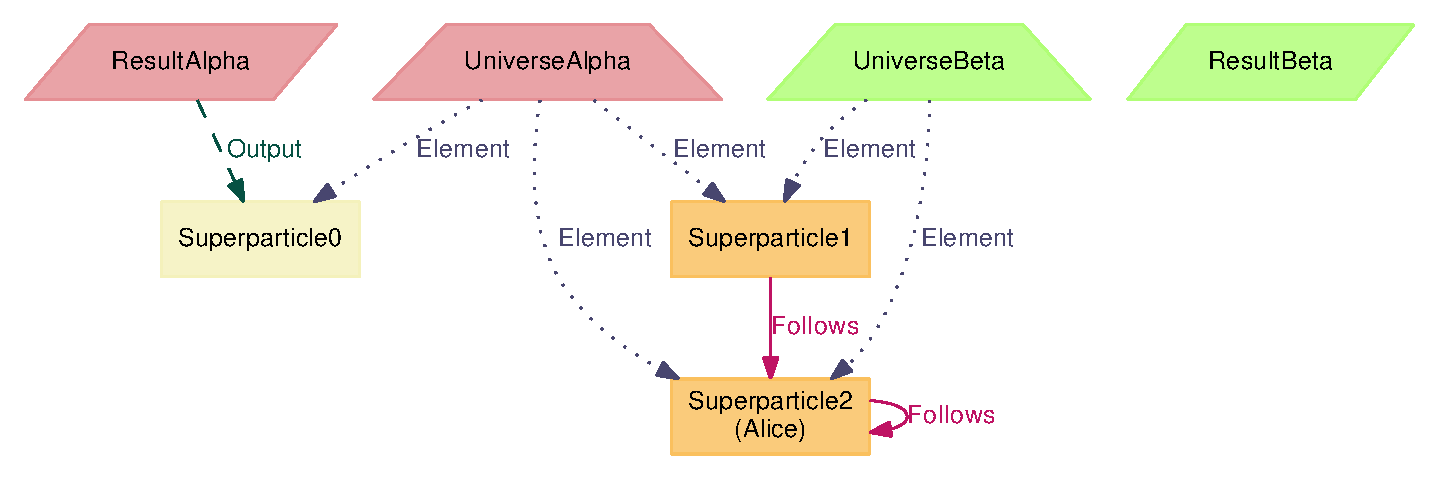
\includegraphics[width=0.99\linewidth]{figures/not-follow-alice.eps}
        \smallskip
        \caption[One counterexample of the Alloy program in \protect{\autoref{src:major-ex1}}.]{
            One counterexample of the Alloy program in \protect{\autoref{src:major-ex1}}. For an extensive explanation of this diagram, see the gray box on \hyperref[fig:not-follow-alice-exp]{page \pageref*{fig:not-follow-alice-exp}}.
        }
        \label{fig:not-follow-alice}
    % \end{mdframed}
    \vspace*{-1pc}
\end{figure}

\begin{figure}[!b]
    \begin{mdframed}[style=standard,innerbottommargin=0pc,skipabove=0pc,skipbelow=0pc]
        \ContinuedFloat
        \caption[One counterexample of the Alloy program in \protect{\autoref{src:major-ex1}}.]{
            One counterexample of the Alloy program in \protect{\autoref{src:major-ex1}}, \emph{continued from \hyperref[fig:not-follow-alice]{page \pageref*{fig:not-follow-alice}}}.

            \captionpar
            In this database model, \mbox{\textcolor[HTML]{48466f}{\dotuline{$\blacksquare$ dotted blue}}} \alloyfn{Element} arrows indicate that the first domain, \alloyfn{UniverseAlpha}, contains three scalar values whereas the second domain, \alloyfn{UniverseBeta}, has only two values (and is incidentally the subset of the first). In addition, \alloyfn{Alice} is another name for \alloyfn{Superparticle2}.

            \captionpar
            The instance of the \rel{Follows} (denoted with \mbox{\textcolor[HTML]{bf1363}{\uline{$\blacksquare$ solid pink}}} \alloyfn{Follows} arrows) contains two rows, namely
                $
                    \;\{\hrsp(\str{Superparticle1},\, \underbrace{\str{Superparticle2}}_\str{Alice}),\; (\underbrace{\str{Superparticle2}}_\str{Alice},\, \underbrace{\str{Superparticle2}}_\str{Alice})\hrsp\}
                $
            This table instance is \emph{valid} because both values \str{Superparticle1} and \str{Superparticle2} belong to \emph{both} domains.

            \captionpar
            The result of query under \alloyfn{UniverseAlpha} is a single row data $\{\str{Superparticle0}\}$ as shown by \mbox{\textcolor[HTML]{065143}{\dashuline{$\blacksquare$ dashed green}}} \alloyfn{Output} dashed arrows). On the other hand, \alloyfn{UniverseBeta} yields empty results.
        }
        \label{fig:not-follow-alice-exp}
    \end{mdframed}
    \vspace*{-1pc}
\end{figure}

\newpage
\begin{lstlisting}[language=alloy,basicstyle={\footnotesize\ttfamily},caption={The complete Alloy program which verifies the query {\protect $Q_\text{\,not\,following\,Alice}$} as shown in \autoref{ex:major-ex1}. Alloy codes highlighted in yellow indicate portions of code which are translated according to and depending on the original database schema and the \textsc{drc} query.},label={src:major-ex1},aboveskip=0pc,belowskip=0pc]
/* Scalar values */
sig Superparticle {} {
	Superparticle = Universe.Element
}

/* Domains */
abstract sig Universe { Element: some Superparticle }
one sig UniverseAlpha, UniverseBeta extends Universe {}

/* Common domain */
some sig Particle in Superparticle {} {
	Particle = UniverseAlpha.Element & UniverseBeta.Element
}

/* Database Instance */
one sig Table {
    <|\hll{ex1table}|>Follows: Particle -> Particle<|\hlr{ex1table}|>
}

/* Constant Values */
one sig Constant {
    <|\hll{ex1alice}|>Alice: Particle<|\hlr{ex1alice}\label{li:alice}|>
}

/* Lists all people who are not following Alice */
fun query[u: Universe]: <|\hll{ex1sig}|>set Superparticle<|\hlr{ex1sig}|> {
    { <|\hll{ex1x}|>x<|\hlr{ex1x}|>: u.Element | <|\hll{ex1pred}|>not (x -> Constant.Alice in Table.Follows)<|\hlr{ex1pred}\label{li:usealice}|> }
}

/* Safety assertion */
assert queryIsSafe {
    all u, u': Universe | query[u] = query[u']
}

/* Results placeholder */
abstract sig Result {
    Output: <|\hll{ex1result}|>set Superparticle<|\hlr{ex1result}|>
}
one sig ResultAlpha, ResultBeta extends Result {} {
    ResultAlpha.@Output = query[UniverseAlpha]
    ResultBeta.@Output = query[UniverseBeta]
}

/* Invoke the verification on the assertion */
check queryIsSafe for 4
\end{lstlisting}

\vspace*{3pc}
\begin{lstlisting}[language=alloy,basicstyle={\footnotesize\ttfamily},caption={The complete Alloy programw which verifies the query {\protect $Q_\text{\,follows\,all\,v2}$} as shown in \autoref{ex:major-ex2}. Alloy codes highlighted in yellow indicates portions of code which are translated according and depending on the original database schema and \textsc{drc} query. Also noted that, unlike \autoref{src:major-ex1}, this Alloy program does not require the \alloy{Constant} model.},label={src:major-ex2},aboveskip=0pc,belowskip=0pc]
/* Scalar values */
sig Superparticle {} {
	Superparticle = Universe.Element
}

/* Domains */
abstract sig Universe { Element: some Superparticle }
one sig UniverseAlpha, UniverseBeta extends Universe {}

/* Common domain */
some sig Particle in Superparticle {} {
	Particle = UniverseAlpha.Element & UniverseBeta.Element
}

/* Database Instance */ <|\label{li:ex2-replace-case1}|>
one sig Table {
    <|\hll{ex2table}|>Follows: Particle -> Particle<|\hlr{ex2table}|>
} <|\label{li:ex2-fix}|>

/* Lists all follows who follows every idols */
fun query[u: Universe]: <|\hll{ex2sig}|>set Superparticle<|\hlr{ex2sig}|> {
    { <|\hll{ex2x}|>x<|\hlr{ex2x}|>: u.Element | <|\hll{ex2pred1}|>all y: u.Element | <|\hlr{ex2pred1}\SuppressNumber|>
        <|\hll{ex2pred2}|>(some z: u.Element | z -> y in Table.Follows) <|\hlr{ex2pred2}|>
        <|\hll{ex2pred3}|>implies (x -> y in Table.Follows)<|\hlr{ex2pred3}\ReactivateNumber|> }
}

/* Safety assertion */ <|\label{li:ex2-replace-case2}|>
assert queryIsSafe {
    all u, u': Universe | query[u] = query[u']
}

/* Results placeholder */
abstract sig Result {
    Output: <|\hll{ex2result}|>set Superparticle<|\hlr{ex2result}|>
}
one sig ResultAlpha, ResultBeta extends Result {} {
    ResultAlpha.@Output = query[UniverseAlpha]
    ResultBeta.@Output = query[UniverseBeta]
}

/* Invoke the verification on the assertion */
check queryIsSafe for 4
\end{lstlisting}

\bigskip
Now let us consider another example, particularly \autoref{ex:follow-all}. In the original scenario, the query $Q_\text{\,follows\,all}$ is unsafe because the universal quantification may probe on domain values which lie outside the database. We are going to fix this query in the next example.

\newpage
\begin{example}
    \phantomsection
    \addcontentsline{toc}{subsection}{Second full example}
    \label{ex:major-ex2}
    Consider the database table $\rel{Follows}(\field{fan},\field{idol})$ and the \textsc{drc} query
    \[
        Q_\text{\,follows\,all\,v2} =
            \{ x \mid \forall y[ \exists z [\rel{Follows}(z, y)] \Rightarrow \rel{Follows}(x, y)] \}
    \]
    By additionally injecting ``$\exists z [\rel{Follows}(z, y)] \Rightarrow$'' into the original query, it \emph{hopefully} guarantees that only idols (represented by $y$) having \emph{at least} one follower in the database are considered. This should disregard the effect of dealing with different domain sets.

    We translated the database schema as well as the above query into the Alloy program as shown in \autoref{src:major-ex2}. However, once Alloy Analyzer was executed, we got unexpected results: it produces counterexamples. After a careful consideration the table \rel{Follows} in every counterexample is empty.

    \marginhead{Using Alloy to debug the query}
    Upon the second glance of the query $Q_\text{\,follows\,all\,v2}$, the result returned by Alloy Analyzer actually makes sense. If the table \rel{Follows} is empty, then the query result would be the same set of people in the domain. \emph{This is one prime example of Alloy could help us finding bugs in the design.}

    We need to fix the program to guarantee that we only considered nonempty table \rel{Follows}, which could be stated as an additional fact towards the \alloy{Table} signature declaration. Therefore, after the closing brace at the beginning of \autoref{li:ex2-fix}, we insert the fact (as highlighted) that the table \alloy{Follows} must contain some (i.e., at least one) rows.

    % FIXME USE THIS INSTEAD OF HARDCODING NUMBERS: \ref*{li:ex2-replace-case1}]}

\begin{lstlisting}[language=alloy,firstnumber=15]
/* Database Instance */
one sig Table {
    Follows: Particle -> Particle
} <|\hll{ex2fact}|>{ some Follows }<|\hlr{ex2fact}|>
\end{lstlisting}

    Once the the modified Alloy program is executed again, it no longer finds a counterexample. Even if we increase the upper limit of the number of each type of model objects from \alloy{4} to \alloy{8}, or even to \alloy{12}, Alloy still does not find a counterexample. Therefore, we may say that ``the \textsc{drc} query $Q_\text{\,follows\,all\,v2}$ \emph{could be} safe, at least as long as the table \rel{Follows} is \emph{nonempty}.''\; This is only a speculation since we could only hope that if Alloy were to find a counterexample, it should have found a small one already.

    \subsubsection*{Alternative Approach}

    Instead of checking for database instances in which the table \rel{Follows} is not empty, we could modify the query to make sure that the \field{fan} must reside in the database. Hence, let us say that the new \textsc{drc} query is
    \[
        Q_\text{\,follows\,all\,v3} =
            \{ x \mid \exists w [\rel{Follows}(x, w)] \wedge \forall y[ \exists z [\rel{Follows}(z, y)] \Rightarrow \rel{Follows}(x, y)] \}
    \]
    The first clause of the conjuction demands that the \field{fan} $x$ must follow at least one person. In other words, that \field{fan} must at least exists in the database.

    The Alloy function implementation of this query can be written as
\begin{lstlisting}[language=alloy,firstnumber=20]
/* Lists all follows who follows every idols */
fun query[u: Universe]: set Superparticle {
    { x : u.Element | <|\SuppressNumber|>
        <|\hll{ex2xtra}|>(some w: u.Element | x -> w in Table.Follows) and <|\hlr{ex2xtra}|>
        (all y: u.Element |
            (some z: u.Element | z -> y in Table.Follows)
            implies (x -> y in Table.Follows))<|\ReactivateNumber|> }
}
\end{lstlisting}
    The only difference between this new code and the original one is shown as highlighted. Everything else remains the same apart from reformatting for clarity.

    When we run this new code, the Alloy Analyzer also does not find any counterexamples, and thus the new query $Q_\text{\,follows\,all\,v3}$ may be safe.
\end{example}

Now that we have established how any simple database schemata and \textsc{drc} queries can be translated into a verification task in Alloy language, in the next section we will experiment with more examples of safe and unsafe queries and see how accurate Alloy performs the verification tasks.

\bigskip
% !TEX root = report.tex
\section{The Experiment}
\label{sec:experiment}

\subsection{Experiment set-up}

In this section, we evaluate how well our proposed Alloy verification framework performs on various \textsc{drc} database queries. Below are the list of database tables in the schema.

\newrobustcmd\Employee{\rel{Employee}}
\newrobustcmd\Supervisor{\rel{Supervisor}}
\newrobustcmd\Reviewer{\rel{Reviewer}}

\begin{itemize}[topsep=0.5pc,itemsep=0.25pc]
    \item  $\Employee(\field{id}, \field{security-level})$:\; each employer ID and their security levels; and
    \item  $\Supervisor(\field{employee-id},\field{boss-id})$:\; stores employee--boss pairs
    \item  $\Reviewer(\field{employee-id},\field{year},\field{reviewer-id})$:\; stores the employee ID of the performance reviewer for each employee in each year
\end{itemize}

\newrobustcmd{\empX}{\ensuremath{x}}
\newrobustcmd{\empY}{\ensuremath{y}}
\newrobustcmd{\boss}{\ensuremath{b}}
\newrobustcmd{\level}{\ensuremath{\ell}}
\newrobustcmd{\yearT}{\ensuremath{t}}

\medskip\noindent
We also consider the following \textsc{drc} queries.

\begin{itemize}[topsep=0.5pc,itemsep=0.25pc]
    \item  $\boldsymbol{Q_1}$\hrsp:\;\marginnote{\textsc{safe}}
        Pairs of employees who share the same boss, and at least one of them has the same security level as their boss.
        \begin{align*}
            Q_1 &= \big\{ \empX, \empY \mid
                \exists \boss \hrsp\big[
                    \Supervisor(\empX, \boss) \wedge \Supervisor(\empY, \boss) \\
            & \qquad\qquad\qquad\wedge \exists \level \hrsp[\Employee(\boss, \level) \wedge (\Employee(\empX, \level) \vee \Employee(\empY, \level))]\big]\big\}
        \end{align*}

    \item  $\boldsymbol{Q_2}$\hrsp:\;\marginnote{\textsc{unsafe}}
        Employees without their own bosses.
        \begin{align*}
            Q_2 &= \big\{ \empX \mid
                \neg \exists \boss \hrsp[\Supervisor(\empX, \boss)] \big\}
        \end{align*}

    \item  $\boldsymbol{Q_3}$\hrsp:\;\marginnote{\textsc{unsafe}}
        Pairs of employees, one of which has the same security level as one of their bosses.
        \begin{align*}
            Q_3 &= \big\{ \empX, \empY \mid
                \exists \boss \exists \level \hrsp[\Employee(\boss, \level) \\
            & \qquad\qquad\qquad\qquad\wedge (\Employee(\empX, \level) \wedge \Supervisor(x, b)  \\
            & \qquad\qquad\qquad\qquad\qquad\vee \Employee(\empY, \level) \wedge \Supervisor(y, b))]\big\}
        \end{align*}

    \item  $\boldsymbol{Q_4}$\hrsp:\;\marginnote{\textsc{safe}}
        Pairs of employees who review each other within the same year.
        \begin{align*}
            Q_4 &= \big\{ \empX, \empY \mid
                \exists \yearT \hrsp[\Reviewer(\empX, \yearT, \empY) \wedge \Reviewer(\empY, \yearT, \empX)] \big\}
        \end{align*}

    \item  $\boldsymbol{Q_5}$\hrsp:\;\marginnote{\textsc{unsafe}}
        \emph{Super} employees who (a) has reviewed everyone else at some point (excluding themselves), and (b) is a boss of at least one employee.
        \begin{align*}
            Q_5 &= \big\{ \boss \mid
                \forall \empX \exists \yearT \hrsp[\Reviewer(\empX, \yearT, \boss)]
                \wedge \exists \empY \hrsp[
                \Supervisor(\empY, \boss) \wedge \neg(\empY = \boss)] \big\}
        \end{align*}
\end{itemize}


\begin{lstlisting}[language=alloy,float,basicstyle={\footnotesize\ttfamily},caption={The complete Alloy program which verifies queries {\protect $Q_1$ through $Q_5$} as defined earlier in \sectionref{sec:experiment}. To verify the safety of other query functions, some portions of the code (shown highlighted) needs to be modified.},label={src:experiment},aboveskip=0pc,belowskip=0pc]
/* Scalar values */
sig Superparticle {} {
	Superparticle = Universe.Element
}

/* Domains */
abstract sig Universe { Element: some Superparticle }
one sig UniverseAlpha, UniverseBeta extends Universe {}

/* Common domain */
some sig Particle in Superparticle {} {
	Particle = UniverseAlpha.Element & UniverseBeta.Element
}

/* Database Instance */
one sig Table {
    Employee: Particle -> Particle,
    Supervisor: Particle -> Particle,
    Reviewer: Particle -> Particle -> Particle
}

/* Query functions */
fun query1[u: Universe]: Superparticle -> Superparticle {
    { x, y: u.Element | some b: u.Element |
        (x -> b in Table.Supervisor) and (y -> b in Table.Supervisor) and
        (some l: u.Element | (b -> l in Table.Employee) and
                             ((x -> l in Table.Employee) or (y -> l in Table.Employee))) }
}
fun query2[u: Universe]: set Superparticle {
    { x: u.Element | not some b: u.Element | x -> b in Table.Supervisor }
}
fun query3[u: Universe]: Superparticle -> Superparticle {
    { x, y: u.Element | some b, l: u.Element |
        (b -> l in Table.Employee) and
        ((x -> l in Table.Employee) and (x -> b in Table.Supervisor) or
         (y -> l in Table.Employee) and (y -> b in Table.Supervisor)) }
}
fun query4[u: Universe]: Superparticle -> Superparticle {
    { x, y: u.Element | some t: u.Element |
        (x -> t -> y in Table.Reviewer) or (y -> t -> x in Table.Reviewer) }
}
fun query5[u: Universe]: set Superparticle {
    { b: u.Element |
        (all x: u.Element | some t: u.Element | x -> t -> b in Table.Reviewer) and
        (some y: u.Element | (y -> b in Table.Supervisor) and not (y = b)) }
}

/* Safety assertion */
assert queryIsSafe {
    all u, u': Universe | <|\hll{exp-assert1}|>query1<|\hlr{exp-assert1}|>[u] = <|\hll{exp-assert2}|>query1<|\hlr{exp-assert2}\label{li:replace-assert}|>[u']
}

/* Results placeholder */
abstract sig Result {
    OneColOutput: set Superparticle,
    TwoColOutput: Superparticle -> Superparticle
}
one sig ResultAlpha, ResultBeta extends Result {} {
    ResultAlpha. <|\hll{exp-alpha-o}\llap{\color{Symbol}@}|>TwoColOutput<|\hlr{exp-alpha-o}|> = <|\hll{exp-alpha}|>query1<|\hlr{exp-alpha}\label{li:replace-alpha}|>[UniverseAlpha]
    ResultBeta. <|\hll{exp-beta-o}\llap{\color{Symbol}@}|>TwoColOutput<|\hlr{exp-beta-o}|> = <|\hll{exp-beta}|>query1<|\hlr{exp-beta}\label{li:replace-beta}|>[UniverseBeta]
}

/* Invoke the verification on the assertion */
check queryIsSafe for 4
\end{lstlisting}

\bigskip
\marginhead{How to verify each specific query}
The Alloy model for these \textsc{drc} queries are shown in \autoref{src:experiment}. By default the Alloy program verifies the query $Q_1$. If we wish to verify other queries, we need to modify some parts of the code (shown highlighted). Specifically,
\begin{itemize}[topsep=0.5pc,itemsep=0.25pc]
    \item  The query function name \alloy{query1} on lines \ref{li:replace-assert}, \ref{li:replace-alpha}, and \ref{li:replace-beta} should be replaced by names of other functions such as \alloy{query2}, \alloy{query3}, etc.
    \item  The result placeholder \alloy{TwoColOutput} may need to be changed to \alloy{OneColOutput} depending of the output signature of the query function.
\end{itemize}

\subsection{Verification result and analysis}

As we expect, Alloy Analyzer has \emph{correctly} determined whether all of these queries are safe. For unsafe queries $Q_2$, $Q_3$, and $Q_5$, Alloy finds the first counterexample in relatively short time (underlined in the output below). The console output for each of these unsafe queries are reproduced here (emphasis added).

\begin{lstlisting}[numbers=none,escapeinside={<|}{|>},xleftmargin=6pc]
<|\llap{\textbf{query2:~~}}|>Executing "Check queryIsSafe for <|\uline{\textbf{10}}|>"
   Solver=sat4j Bitwidth=0 MaxSeq=0 SkolemDepth=1 Symmetry=20
   4658 vars. 1464 primary vars. 6953 clauses. 15ms.
   <|\uline{Counterexample} \uline{found}|>. Assertion is invalid. <|\uline{\textbf{17ms}}|>.
\end{lstlisting}

\begin{lstlisting}[numbers=none,escapeinside={<|}{|>},xleftmargin=6pc]
<|\llap{\textbf{query3:~~}}|>Executing "Check queryIsSafe for <|\uline{\textbf{10}}|>"
    Solver=sat4j Bitwidth=0 MaxSeq=0 SkolemDepth=1 Symmetry=20
    38148 vars. 1464 primary vars. 128213 clauses. 2068ms.
   <|\uline{Counterexample} \uline{found}|>. Assertion is invalid. <|\uline{\textbf{189ms}}|>.
\end{lstlisting}

\newpage
\begin{lstlisting}[numbers=none,escapeinside={<|}{|>},xleftmargin=6pc]
<|\llap{\textbf{query5:~~}}|>Executing "Check queryIsSafe for <|\uline{\textbf{10}}|>"
   Solver=sat4j Bitwidth=0 MaxSeq=0 SkolemDepth=1 Symmetry=20
   9498 vars. 1464 primary vars. 24953 clauses. 58ms.
   <|\uline{Counterexample} \uline{found}|>. Assertion is invalid. <|\uline{\textbf{99ms}}|>.
\end{lstlisting}

\noindent
For safe queries $Q_1$ and $Q_4$, here is the console output (emphasis added).

\begin{lstlisting}[numbers=none,escapeinside={<|}{|>},xleftmargin=6pc]
<|\llap{\textbf{query1:~~}}|>Executing "Check queryIsSafe for <|\uline{\textbf{10}}|>"
   Solver=sat4j Bitwidth=0 MaxSeq=0 SkolemDepth=1 Symmetry=20
   32858 vars. 1464 primary vars. 105823 clauses. 457ms.
   <|\uline{No} \uline{counterexample} \uline{found}|>. Assertion may be valid. <|\uline{\textbf{16593ms}}|>.
\end{lstlisting}

\begin{lstlisting}[numbers=none,escapeinside={<|}{|>},xleftmargin=6pc]
<|\llap{\textbf{query4:~~}}|>Executing "Check queryIsSafe for <|\uline{\textbf{10}}|>"
   Solver=sat4j Bitwidth=0 MaxSeq=0 SkolemDepth=1 Symmetry=20
   7898 vars. 1464 primary vars. 17663 clauses. 39ms.
   <|\uline{No} \uline{counterexample} \uline{found}|>. Assertion may be valid. <|\uline{\textbf{132ms}}|>.
\end{lstlisting}

\begin{note}
    In terms of computational cost,
    \begin{itemize}[topsep=0.5pc,itemsep=0.25pc]
        \item  Queries with more complex syntax tend to take more time to verify (cf.\ \alloy{query1} vs.\ \alloy{query4}) even if the maximum numbers of objects for each type in the search space are the same.
        \item  When comparing queries with similar complexity (such as \alloy{query1} vs.\ \alloy{query3}), unsafe queries take less computation time as it only requires to find one counterexample whereas safe queries need to exhaust the search space.
    \end{itemize}
    In addition, if we choose to vary the maximum number of objects for each model type in Alloy verification task, then undoubtedly, as the number increases, the computational cost also increases. This is a normal Alloy behavior so we would not include the result of such experiment here.
\end{note}

\bigskip
% !TEX root = report.tex
\section{Conclusion}

So far we have established that we could use Alloy Analyzer to verity if a \textsc{drc} query is safe under a given database schema. For future work, we could implement a translator to automate the verification process; that is, given as input the database specification and the query compatible with relational calculus, the translator converts the input into Alloy programming syntax to be verified by Alloy Analyzer.

On the other hand, the presented framework itself is still limited as it could deal only with a small subset of what \textsc{drc} queries are capable of. Here are the list of features which could be added in this project in the future.
\begin{itemize}[topsep=0.5pc,itemsep=0.25pc]
    \item  \textbf{Support for all scalar value comparison operators.}\; In this project, the only allowed operation between one or more scalar values is the equality comparison operator ($=$). This does not fully reflect the behavior of the domain in real world.

        One possible improvement is to make sure that \alloy{Superparticle}s are totally ordered so that other comparison operators such as $<$ and $\geq$ would work. On the same note, we should also be able to refer to primitive constant values, particularly the maximum and minimum values in the domain.

        This should be relatively easy to implement since there is an undocumented Alloy library which supports total ordering out of the box. This improvement will make operations such as number comparison possible to model.

    \item  \textbf{Support for bounded and unbounded integers.}\; This is an extended improvement over the previous point. However, this should be much more complicated since the support for integers in Alloy is very limited, apart from basic arithmetic operations like addition, subtraction, etc.

    \item  \textbf{Support for functional dependencies in database schema.}\; Functional dependency in a database systems enforces the values of some columns of data based on other columns. For example, the table $\rel{GeoData}(\field{city},\field{state},\field{zipcode})$ may have the functional dependency
        \[
            \field{zipcode} \mapsto \field{city},\field{state}
        \]
        That is, based on \field{zipcode} alone, there is a unique \field{city} and a unique \field{state} in the table \rel{GeoData}.

        This improvement will greatly benefit the query safety verification because (a) modeling functional dependency also implies modeling of primary keys, candidate keys, unique keys etc., and (b) the safety of \textsc{drc} queries also depends on functional dependencies.

        The modeling of functional dependencies in Alloy should be simple at least for tables with at most two columns. For tables with three or more columns, being able to specify the multiplicity between columns is much more complicated.

\end{itemize}

% \medskip
% On a slightly related note, it might be possible to expand the proposed verification framework to verify whether a \textbf{Datalog} querying syntax is safe. Datalog is another database query language similarly to relational calculus but with two notable differences: (1) Datalog instead uses Prolog-style, rule-based syntax, and (2) Datalog supports recursion in data model, which makes it more expressive than relational calculus \cite{Ullman:1988:PDK:42790}.



\begin{center}
    \adforn{21}\quad\adforn{11}\quad\adforn{49}
\end{center}

% \appendix
% \input{chap_additional.tex}

\newpage
\bibliographystyle{alpha}
\bibliography{refs}

\end{document}
